\documentclass[conference]{IEEEtran}
\IEEEoverridecommandlockouts
% The preceding line is only needed to identify funding in the first footnote. If that is unneeded, please comment it out.
\usepackage{cite}
\usepackage{amsmath,amssymb,amsfonts}
\usepackage{algorithmic}
\usepackage{graphicx}
\usepackage{textcomp}
\usepackage{xcolor}
\usepackage{subcaption}
\usepackage{hyperref}
\usepackage{float}
\def\BibTeX{{\rm B\kern-.05em{\sc i\kern-.025em b}\kern-.08em
    T\kern-.1667em\lower.7ex\hbox{E}\kern-.125emX}}
\begin{document}

\title{Camouflaged Animal Detection}

    
\author{\IEEEauthorblockN{Khubaib Naeem Kasbati}
\IEEEauthorblockA{
Department of Computer Science \\
Habib Univeristy - Karachi, Pakistan \\
kk04333@st.habib.edu.pk}
\and
\IEEEauthorblockN{Qazi Muhammad Talha}
\IEEEauthorblockA{
Department of Computer Science \\
Habib Univeristy - Karachi, Pakistan \\
qt05099@st.habib.edu.pk}
\and
\IEEEauthorblockN{Muhammad Munawwar Anwar}
\IEEEauthorblockA{
Department of Computer Science \\
Habib Univeristy - Karachi, Pakistan \\
ma04289@st.habib.edu.pk}
}


\maketitle

\begin{abstract}
As a part of their evolutionary trait, a lot of animals have learned to conceal themselves in their surroundings in order to hide from their prey or predator. They do this by various methods including background matching, imitating color and
pattern of the environment, and disguising body outlines\cite{price2019background}. 
The ability to seamlessly blend into their surroundings poses a challenge when it comes to detection and differentiation from the background. Known as Camouflaged Object Detection (COD), it is one of the most challenging task in the domain of computer vision, since the target object and background have many similarities \cite{9156837}. Another thing that makes COD challenging is limited availability of annotated data. We aim to resolve this by making a unified dataset consisting of existing data-sets such as COD10K, MoCA, CHAMELEON and CAMO. Our objective is to train state of the art object detection techniques such as Y0LOv5 on the unified dataset and then evaluate the model using mean Average Precision (mAP).

\end{abstract}

\begin{IEEEkeywords}
Computer Vision, Camouflaged Object Detection (COD), YOLOv5, Animal Classification.
\end{IEEEkeywords}

\section{INTRODUCTION}
COD is a growing sub-field under the heading of computer vision as it has various applications in medical imaging, animal tracking and animal behavior. Since animals are one of the prime examples present in terms of camouflaged objective, there exist a lot of variation within the samples that we go through as different animals tend to camouflage themselves in different ways \cite{price2019background}. This vast variation in the data shall bring up a lot of challenges, hence makes this task a representative example that will enable us to go a long way to tackle the issue of COD.


Unlike the standard object detection tasks, which has seen significant progress 
in recent years, COD poses some unique challenges, particularly due to the lack of large-scale 
annotated datasets. While Deep Learning based object detection methods have seen significant 
progress in recent times, they have required large-scale labeled datasets such as MS-COCO \cite{coco}
(more than 2 million instances). Unfortunately, COD datasets are much more limited in the 
number of annotated samples such as the COD10k (5066 labeled samples) \cite{ConcealedFan} and MoCA 
(37000 labeled frames from 141 videos) \cite{Lamdouar_2020_ACCV} datasets.
Previous methods in the domain have taken a model-centric approach, aiming to 
optimally utilize the limited annotated data, pioneering novel methods in unsupervised and semi-
supervised learning. These methods use complex models that are especially attuned to learning 
with limited samples. However, while making the best use of the smaller datasets, such 
methods fail to match the performance of fully supervised methods trained using large-scale 
datasets. Therefore, this research proposes to take a more data-centric approach to the 
problem rather than the previously used model-centric methods.

Since the biggest concern is data, the project for us begins by first gathering and stitching together various sources (including the ones mentioned above) of camouflaged animal data into one large dataset. Data labels would be in the YOLOv5 format. Moreover, the second part of the project entails conducting a thorough literature review into firstly, these datasets and secondly, COD techniques in general and thirdly, state of the art Standard Object Detection Techniques. The final objective is to train a state-of-the-art object detector using the unified dataset and report mean Average Precision (mAP). This detector will serve as the base model to compare against detection being done through synthetic images.


% The characteristic features of this project are listed as follows:
% \begin{itemize}
%     \item One of the biggest challenges that is faced in Deep Learning based Camoflauged Object Detection Tasks is the lack of large-scale annotated datasets. This project collect existing datasets and creates a unified dataset which serves as a benchmark dataset for other state of the art Camouflage Object Detection Techniques.
%     \item Camouflaged Object Detection has several uses in military, agriculture, medical, and environmental protection (e.g. find rare species in a search and rescue). Methods that work well in the detection of camouflaged animals can subsequently be evaluated in other domains.
% \item It can be used to improve how search engines perform with reverse image search. For example, currently their classifier might not be able to detect the camouflaged animal. With COD, it might be able to and can give better results. \cite{9156837}
% \end{itemize}



\section{LITERATURE REVIEW}
\subsection{EXISTING COD DATASETS}
There mainly exist four COD datasets, namely the \textbf{CAMO}, \textbf{CHAMELEMON}, \textbf{COD10K} and \textbf{MoCA}. The CHAMELEON is an unpublished dataset that has 76 images downloaded from the Internet for testing. The CAMO dataset  includes 1,250 camouflaged images divided into eight categories, where 1,000 camouflaged images are for training, and the remaining 250 images are for testing \cite{le2019anabranch}. Most of the dataset images are mammals, insects, birds, and aquatic animals, each with approximately similar proportions, and a small number of reptiles, human art, soldiers, and amphibians. The dataset is very diverse making it adaptable but due to insufficient samples, augmentation is used to increase the samples. Deng-Ping Fan et al. \cite{9156837}  provided a more challenging dataset, named COD10K.
It contains 10,000 images divided into 78 camouflaged object categories such as aquatic, flying, amphibians, and terrestrial. This dataset also consists of many high-resolution images. Moreover, this dataset provides rich labels including edge object instances and bounding boxes annotations which can also facilitate many vision tasks such as localization, object proposal, semantic edge detection, etc. To ensure high-quality annotation three viewers were invited to participate in the labelling process for 10-fold cross-validation. MoCA stands for Moving Camouflaged Object Dataset \cite{DBLP:journals/corr/abs-2011-11630}. It contains 141 videos and 37K Frames. Further, they provide the largest testing dataset with 4,121 images for effective model evaluation. Furthermore, it contains 67 categories and provides both bounding box annotations and motion type labels. Other datasets were also  proposed, but they have a limited number of samples. Bideau et. al. \cite{DBLP:journals/corr/BideauL16} proposed a camouflaged animal video dataset but the dataset has only 9 videos with animals consisting in a third of the content.


\subsection{MODEL-CENTRIC APPROACHES }
In early research, most methods use low-level features, including texture and edges, to discriminate objects from the background. However, these methods fall into the trap of camouflage, as the low-level features are disrupted in camouflage to deceive prey/predators. Therefore, new models resort to deep networks to recognize the more complex properties of camouflage. Among those, Le et al. \cite{le2019anabranch} introduced the joint image classification and camouflaged object segmentation framework. Yan et al. \cite{yan2021mirrornet}  presented an adversarial segmentation stream using a flipped image as input to enhance the discriminative ability of the main segmentation stream for camouflaged object detection. Fan et al. \cite{9156837} proposed SINet to gradually locate and search for the camouflaged object.


Le et al. \cite{le2019anabranch}  proposed the end-to-end network: Anabranch Network, which leverages both classification and segmentation tasks for Camouflage Object Detection.  In nature, once a predator has an awareness of camouflaged prey in the scene then it can attempt to localize it for hunting. This utilizing of the awareness of the prey as a prior is an essential cue used for camouflaged object segmentation by Anabranch Network (ANet). It leverages the advantages of the classification stream and the segmentation stream, in order to segment camouflaged objects. The classification stream is used as awareness of existing of camouflaged object(s) in an image (like predators). This is done since there is no guarantee whether a camouflaged object is there or not. Only if it exists, the object(s) should be accurately segmented. Otherwise no segmentation is necessary. 


Recently, Le et al. \cite{DBLP:journals/corr/abs-2103-17123} explored the camouflaged instance segmentation by training Mask RCNN on CAMO dataset. Differently from the state-of-the-art ANet, where classification stream and segmentation stream are applied on the whole image, in this work, we first obtain object proposal, then we apply segmentation on each object proposal.



In MirrorNet \cite{yan2021mirrornet}, a bio-inspired mirror-stream is used to guide the network for camouflage object segmentation. The mirror-stream (flipped stream) is useful as when we flip the images, humans are then not as eaily fooled by the natural settings and notice differences in the images. Therefore, the flipped images accidentally break the natural layout which leads to the larger distance between the background and the camouflaged objects. This allows MirrorNet variants to yield better results than all state-of-the-art methods tested in the paper. This paper adopts the CAMO dataset which was proposed and bench marked by the previous state-of-the-art camouflaged object segmentation model, for the training of instance segmentation framework.

Deng-Ping Fan et al. \cite{9156837} provided a comprehensive study about camouflaged object detection. There are three main contributions in this study. The first major contribution is a large scale dataset, COD10K. The second major contribution is a baseline model SINet which consists of two main components: Receptive Field (RF) and Partial Decoder component (PDC). SINet model emulates the first two stages of hunting, i.e., search and identification. Specifically, the former phase is responsible for searching for a concealed object, while the latter one is then used to precisely detect the concealed object in a cascaded manner.  Once an image is input, SINet leverages a densely connected strategy to preserve more information from different layers and then uses the modified RF component to enlarge the receptive field. Then the input is passed to the attention module and the process is repeated to obtain the final result. The standard cross-entropy loss to was used to train the SINet. SINet along with various baselines was evaluated on the COD10K dataset and SINet achieved state-of-the-art performance across all evaluation metrics. The third main contribution is highlighting the potential applications of SINet. This study highlights that new techniques such as weakly supervised learning, zero-shot learning, VAE, and multi-scale backbone could also be explored. Furthermore, in the future COD10K can be extended dataset to provide input of various forms, for example, RGB-D camouflage object detection among others.

Deng-Ping Fan et al. \cite{ConcealedFan} is an extension of the conference version \cite{9156837} in terms of several aspects. This paper provides a more detailed analysis of the COD10K dataset, including the taxonomy, statistics, annotations, and resolutions. Secondly, this paper presents an improved SINet model by introducing neighbour connection decoder (NCD) and group-reversal attention (GRA). The three main components of SINet are: NCD which is responsible for providing the location information, GRA blocks which work collaboratively to refine the coarse prediction from the deeper layer  and texture enhanced module (TEM which is used to capture fine-grained textures with the enlarged context cues). The loss function is defined as the sum of the weighted intersection-over-union (IoU) loss and binary cross entropy (BCE) loss for the global restriction and local (pixel-level) restriction. The models were evaluated on the whole CHAMELEON dataset and the test sets of CAMO and COD10K.This work can be extended in the future by automatically searching the optimal receptive fields and employing improved feature representations for a better model performance.

Fan Yang et al. \cite{9710683} presents a novel approach using a probabilistic representational model in combination with transformers to explicitly reason under uncertainties, namely uncertainty-guided transformer reasoning (UGTR), for camouflaged object detection. The core idea is to learn a conditional distribution over the backbone’s output to obtain initial estimates and associated uncertainties, and then reason over these uncertain regions with an attention mechanism to produce final predictions. This approach combines the benefits of both Bayesian learning and Transformer-based reasoning, allowing the model to handle camouflaged object detection by leveraging both deterministic and probabilistic information. The UGTR is composed of three main components: uncertainty quantification network (UQN), uncertainty-induced transformer (UGT) and auxiliary prototyping transformer (PT). The UQN is a probabilistic representational model to capture the uncertainty for camouflaged object detection and it contains two parts: feature extractor (backbone) $F_{\theta_1}$ and probabilistic module $F_{\theta_2}$ which models the variance of the backbone’s output as a measure of uncertainty.  The loss function used to train the UQN is a weighted combination of a standard BCE loss and a Kullback-Leibler (KL) divergence. In addition to the uncertainty, the high-level, global context information also plays a critical role in decamouflaging. However, for the task of camouflaged object detection, the conventional techniques, such as global average pooling, are not reliable due to texture similarities between camouflaged objects and the background. This problem is tackled using metric learning  and a PT is used to obtain representative and discriminative prototypes. UGRM (uncertainty-guided random masking) is added to the UGT to focus on uncertain (difficult) regions during training. It works as a hard-example-mining module, which induces the UGT to focus on difficult (uncertain) regions during training. The UGTR achieves state-of-the-art (SOTA) performance on the CHAMELEON, CAMO and COD10K without requiring any extra information (e.g., fixation or boundary).  In addition, only the pixel-wise labels are used for model training.


Existing COD models are built upon binary ground truth to segment the camouflaged objects but this fails to take into account the level of camouflage. This is important since some parts of the camouflaged objects make them easily detectable by predators.  Yunqiu and Jing et. al \cite{lv2021simultaneously} propose that understanding the level of camouflage can help to design more sophisticated camouflage techniques. Their primary contribution  is to propose the first ranking based COD network (Rank-Net) to simultaneously localize, segment and rank camouflaged objects. The localization model finds discriminative regions that make the object's presence obvious. The segmentation model then segments the full scope of the camouflaged objects and the ranking model infers the detectability of different camouflaged objects. Ranknet uses ResNet50 as a backbone to extract features and then Feature Pyramid Network (FPN)  is employed to integrate the feature maps of different levels. Then the Region Proposal Network (RPN) is adopted, which takes the feature of the whole image as input, and detects the regions that are likely to contain the camouflaged instances, i.e. the regions of interest (ROIs). The RPN consists of two branches: a classification branch, which determines whether the candidate bounding box contains the camouflaged object; and 2) a regression branch, which regresses the coordinates of the ground truth camouflaged object bounding box. With features produced by FPN, the ROIAlign module is used to extract feature maps of the ROIs. Then, we predict the rank and regress the location of the camouflaged object, respectively. Finally, features of the detected camouflaged object are fed into a segmentation branch to output a binary mask for each camouflaged instance.

Using image enhancement, Ce and Xinyu et al \cite{last} distinguish between image and object using a method known as CLAHE (Contrast Limited Adaptive Histogram Equalization). This method enlarges the similarity between target and background, enhances the significance of target texture and color feature, and improves target feature recognition. Moreover, the authors propose using a deep neural network model to detect the target. They utilize RPN to directly generate candidate regions, and use Fast R-CNN for border regression and attribute classification. The data used in the study is of leaves and chameleons.

Shuai and Dinei et. al. \cite{8297083}  focused on foreground object detection in camouflaged scenarios by extracting texture features. It utilizes a technique known as Texture Guided Weighted Voting (TGWV) in order to separate foreground objects using the stationary wavelet transform. This method breaks down an image into 4 frequency bands; LL, LH, HL, and HH. These frequency bands are based on different frequency approximations (LL being low and the rest being high) and in different directions (LH = horizontal/ HL = vertical/ HH = diagonal). This wavelet decomposition results in various small differences in each of the different frequencies that have been generated. In terms of the methodology, the authors of this papers first employ a background modelling process such as GMM in MOG2 to form the background image. Then the stationary wavelet transform is used to break down the image into various levels of wavelet bands. Then the difference is calculated to compare each current image (after wavelet decomposition) and the background image (also after wavelet decomposition). And finally, a weighted voting scheme is used to separate the foreground object using three different weight mechanisms. This process is summarized in figure \ref{fig1}.
\begin{figure}[h]
    \centering
    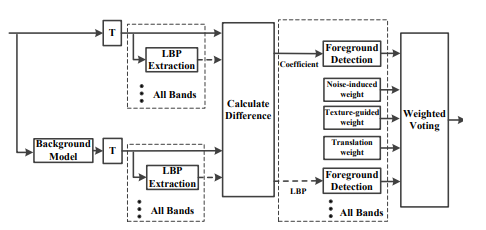
\includegraphics[width=0.7\linewidth]{1.png}
    \caption{Wavelet Transform}
    \label{fig1}
\end{figure}
\newpage
In conclusion, the paper uses 5 grayscale video sequences of resolution $ 1536\times 1152 $ in real scenes of people wearing clothes similar to their surroundings and after applying the proposed method of foreground object detection, they obtain a recall of 0.98, a precision of 0.89 and an F-Measure of 0.93. This performance is better than most foreground extraction algorithms that it has been compared against by the authors (such as just MOG2 and SuBSENSE).

Zheng and Xiongwei et. al. \cite{ 10.1145/3321408.3326662} propose a strong semantic dilation network (SSDN) to detect camouflaged people. The data set used is made by the authors and contains 2600 images ($854 \times 854$) of camouflaged people in 26 different patterns of camouflage. Each picture also has a corresponding pixelwise ground-truth map. The SSDN that has been proposed in the paper consists of 3 parts. It is made by combining VGG Net, with a Semantic Information Enhancer and then an Up-sample and Dilation part. The process is summarized in the figure \ref{fig2}.
\begin{figure}[h]
    \centering
    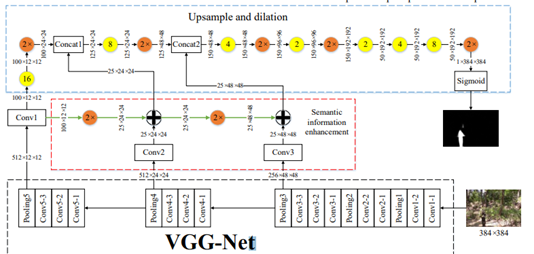
\includegraphics[width=\linewidth]{2.png}\\
    \caption{SSDN}
    \label{fig2}
\end{figure}
\newline
Therefore, as visible from the network, the feature maps from the deeper layers (Pooling 3,4,5) are passed through 1x1 conv layers (Conv1,2,3) and then up-sampled and added together to increases the amount of semantic information obtained. Then a principle of dilated convolutions is used to enlarge the receptive field by up-sampling the feature maps (using de-convolutional layers). The results show better performance in comparison to traditional hand-crafted feature selection models such as CGVS, HDCT and DRFI. In conclusion the paper claims SSDN can detect camouflage people fast and accurately.


\subsection{STANDARD SOA OBJECT DETECTION MODELS}
There are two types of Object Detection Models: Single Stage Detector and Two Stage Detector. A Single State Detector is a type of object detection model that skips the region proposal stage of two-stage models and runs detection directly over a dense collection of regions. They are quicker than two-stage detectors but less precise. YOLO is an example of a single stage detector (You Only Look Once) \cite{DBLP:journals/corr/RedmonDGF15}. On the other hand, Two Stage Detector is a type of object detection model that separates object detection into two stages. One model is used to generate region proposals, while a second model is use to classify these regions and refine the object's localisation. They are more accurate yet slower than single stage detectors. Faster R-CNN is an example of a two-stage detector \cite{1}. The standard state of the start Object Detection models that we will be covering in this section are: Fast R-CNN, Faster R-CNN, DETR, VarifocalNet, YOLO, YOLOv5, YOLOX and YOLOF.

% Please add the following required packages to your document preamble:
% \usepackage{graphicx}
% Please add the following required packages to your document preamble:
% \usepackage{graphicx}
% Please add the following required packages to your document preamble:
% \usepackage{graphicx}
\begin{table}[h]
\centering
\resizebox{\linewidth}{!}{%
\begin{tabular}{|ll|}
\hline
\multicolumn{2}{|c|}{Mean   Average Precision on the MS-COCO Dataset} \\ \hline
\multicolumn{1}{|l|}{Model} & mAP \\ \hline
\multicolumn{1}{|l|}{Fast R-CNN \cite{3}} & 35.9 \\ \hline
\multicolumn{1}{|l|}{Faster R-CNN \cite{1}} & 38.6 \\ \hline
\multicolumn{1}{|l|}{DETR-DC5-R101 \cite{2}} & 44.9 \\ \hline
\multicolumn{1}{|l|}{VarifocalNet \cite{4}} & 55.1 \\ \hline
\multicolumn{1}{|l|}{YOLO \cite{DBLP:journals/corr/abs-2103-17123}} & 57.9 \\ \hline
\multicolumn{1}{|l|}{YOLOF \cite{5}} & 60.5 \\ \hline
\multicolumn{1}{|l|}{YOLOX \cite{6}} & 47.3 \\ \hline
\multicolumn{1}{|l|}{YOLOv5s \cite{glenn_jocher_2021_5563715}} & 56.8 \\ \hline
\end{tabular}%
}
\caption{A summary of the mAP acheived by different models on the MS-COCO Dataset.}
\label{tab:my-table1}
\end{table}


Ross \cite{3} proposed a new method, Fast R-CNN  for identifying objects using deep convolutional networks. The model diagram of Fast R-CNN can be see in Figure \ref{fig3}. Fast R-CNN is faster than other methods, more accurate, and can identify more object classes. The network first processes the whole image with several convolutional layers to produce a conv feature map. Moreover, a region of interest pooling layer extracts a fixed-length feature vector from the feature map for each object proposal. Each feature vector is fed into a sequence of fully connected layers that break into two output layers. The first one produces softmax probability estimates over object classes and a background class. The second layer outputs four real-valued numbers for each of the object classes. These numbers encode refined bounding-box positions for one of the object classes. The paper also presents detailed experiments that suggest sparse object proposals improve detector quality.
\begin{figure}[h]
    \centering
    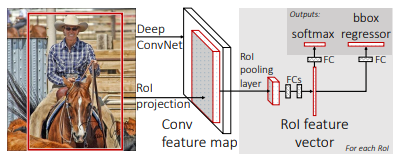
\includegraphics[width=\linewidth]{3..png}\\
    \caption{Fast R-CNN}
    \label{fig3}
\end{figure}
\newpage
Shaoqing and Kaiming et. al \cite{1} introduces a new network, called a Region Proposal Network (RPN), also referred to as Faster R-CNN. The model diagram of Fast R-CNN can be see in Figure \ref{fig4}. This network shares features with the detection network, which means it doesn't cost anything extra to use. The RPN is a mini-network that is implemented with an n×n convolutional layer followed by two sibling 1×1 convolutional layers. It takes an image as input and outputs a set of rectangular object proposals, each with an objectness score. The RPN is trained to generate good region proposals, which are then used by Fast R-CNN for detection. By sharing convolutional features with the down-stream detection network, the region proposal step is nearly cost-free. This method enables a unified, deep-learning-based object detection system to run at near real-time frame rates. The learned RPN also improves region proposal quality and thus the overall object detection accuracy. 
\begin{figure}[h]
    \centering
    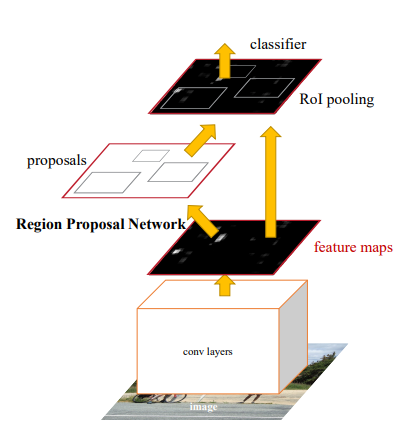
\includegraphics[width=\linewidth]{1..png}\\
    \caption{Faster R-CNN}
    \label{fig4}
\end{figure}

The DETR \cite{2} utilizes a simpler approach and treats the task as a direct set prediction problem. The model diagram of DETR can be see in figure \ref{fig5}. This means that the system will try to predict a set of objects, rather than just one, and that it will do so in a single pass. The system makes use of bipartite matching and is made up of a CNN backbone, an encoder-decoder transformer, and a simple feed forward network. These components work together to take an image and turn it into predictions for what objects are in that image. DETR has been shown to be on par with other, more established object detection systems such as the Faster R-CNN, and has the potential to be even better with some more work. 
\begin{figure}[h]
    \centering
    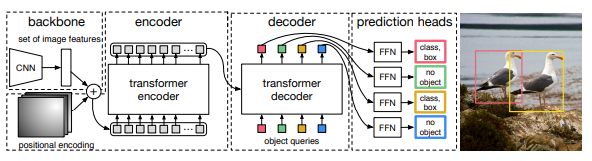
\includegraphics[width=\linewidth]{2..png}\\
    \caption{DETR}
    \label{fig5}
\end{figure}
\newline
VarifocalNet \cite{4} is a dense object dectector. It is based on the FCOS+ATSS structure, but with some important changes. Firstly, it utilizes a new loss function known as the varifocal loss. This loss function is used to train the detector to predict the Iou-aware Classification Score (IACS). Secondly, we a novel star-shaped bounding box feature representation is proposed. This representation is used for both IACS prediction and bounding box refinement. Finally, VarifocalNet also incorporates a new branch in the detector that is used for bounding box refinement. This branch takes as input the initial bounding box and the feature map, and outputs the refined bounding box. On MS COCO, VarifocalNet using the best model of the paper ``VFNet-X-1200 with Res2Net-101-DCN'' achieves a mAP of 55.1 on the COCO test-dev. This mAP holds up to the competing latest optimized object detectors.


YOLO \cite{DBLP:journals/corr/RedmonDGF15} is a single-stage object detection model. Object detection is framed as a regression problem to spatially separated bounding boxes and associated class probabilities. A single neural network predicts bounding boxes and class probabilities directly from full images in one evaluation. Since the whole detection pipeline is a single network, it can be optimized end-to-end directly on detection performance. The network uses features from the entire image to predict each bounding box. It also predicts all bounding boxes across all classes for an image simultaneously. This means the network reasons globally about the full image and all the objects in the image.

\begin{figure}[h]
    \centering
    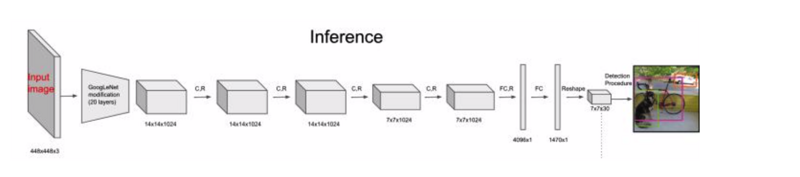
\includegraphics[width=\linewidth]{3667085056-5c21a39288e97_articlex.png}\\
    \caption{YOLO}
    \label{fig7}
\end{figure}

You Only Look One-level Feature (YOLOF) \cite{5} is a simpler and more efficient method for addressing the optimization problem in dense object detection, without using FPN (Feature Pyramid Networks). YOLOF is made up of three parts: the backbone, the encoder, and the decoder. The backbone is a pre-trained feature that is used to detect objects. The encoder is used to cover all objects on various scales. The decoder is used to generate classification scores for all predictions. It performs better than RatinaNET and DETR and could be used to serve as a baseline model for single stage dectectors. The model diagram for YOLOF can be seen in figure \ref{fig6}.
\begin{figure}[h]
    \centering
    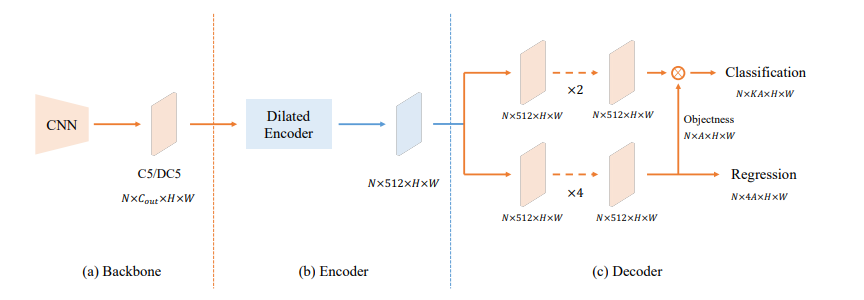
\includegraphics[width=0.7\linewidth]{5..png}\\
    \caption{YOLOF}
    \label{fig6}
\end{figure}

The YOLOv5 \cite{glenn_jocher_2021_5563715} is a Pytorch Implementation of the YOLO model by Glenn Jocher under 
\href{https://github.com/ultralytics}{Ultralytics organization on GitHub}. It is in itself a collection of object detection models. Starting from very small models, capable of giving real-time FPS on edge devices to very large and accurate models meant for cloud GPU deployments. The smallest and the fasted model is YOLOv5 nano (YOLOv5n) whereas the largest and the slowest model is YOLOv5 extra large (YOLOv5x). Unlike many object detection models use predefined anchor boxes according to the MS COCO dataset, YOLOv5 uses a genetic algorithm to generate the anchor boxes. This process is called autoanchor, which recomputes the anchor boxes to fit the data if the default ones are not good. It is used in conjunction with the k-Means algorithm to create k-Means evolved anchor boxes. Consequently, YOLOv5 works so well even on varied datasets.

Zheng and Songtao et. al \cite{6} bring some improvements to the YOLO series of detectors and propose a new high-performance detector called YOLOX. YOLOX is switched to an anchor-free manner and other advanced detection techniques, are used to achieve state-of-the-art results across a large scale range of models. It is trained using stochastic gradient descent, with a learning rate that is linearly scaled to the batch size. The weight decay is set to 0.0005, and the SGD momentum is set to 0.9. The batch size is 128 by default and the input size is drawn from 448 to 832, with 32 strides. The advanced detection techniques allow YOLOX to achieve a better trade-off between speed and accuracy than other models.





\section{METHODLOGY}
\subsection{FINAL DATASET}
The final dataset was created by merging only those images in the COD10K and MoCA Dataset whose annotations were given. The final dataset consists of 12,683 RGB Images all of which were resized to a size of $416 \times 416$. 5066 Images belong to the COD10K Dataset and 7617 belonging to the MoCA dataset. The merged dataset contains 126 different categories of animals with 57 belonging only to MoCA, 59 belonging only to the COD10K and 10 categories belonging to both datasets. During the merging of the two datasets, we ensured that each class was assigned only one index. To enforce this, we traversed the MoCA Dataset and created a list of classes along with their index. Then for all the classes in the COD10K, we assigned a unique index if and only if that particular class was not already assigned an index during the traversal of the MoCA Dataset. In case of the MoCA Dataset, we were given an annotations.csv file which had the bounding box for each object in the COCO format. However, in case of the COD10K Dataset, a binary mask was given instead of the BBOX. Consequently, for all the images in COD10K Dataset, the bounding box for each image was found by using the minimum enclosure bounding box. All the images where renamed to the form $\langle i \rangle \text{.jpg}$ and their labels were stored in the file $\langle i \rangle \text{.txt}$ where $ i \in [0,12682]$.   Each row in the $\langle i \rangle \text{.txt}$ file contained the label and BBOX for one object. Since we are using a YOLO detector, each row in the file $\langle i \rangle \text{.txt}$ was of the format: $\langle idx \rangle \langle xcenter \rangle \langle ycenter \rangle \langle w \rangle \langle h \rangle$ where xcenter is the x-coordinate of the center of the BBOX, ycenter is the y-coordinate of the the center of the BBOX, idx is the class index and w,h are the weight and height of the bounding box. All of these were normalized between 0 and 1.0.  

\subsection{TRAIN TEST SPLIT}
The train-test split that we decided was 80 percent train and 20 percent test. In order for our model to give optimal results, we had to ensure the train test split was balanced. Consequently, instead of doing the train test split after the merging the dataset, we performed the train test split on each dataset individually and then merged them. For MoCA dataset, if there were multiple videos for the same animal then the split was made on videos. However, if there was only one video for an animal, then the split was made on the image frames from the video. The total number of number training images was equal to 9750 with 4028 Images coming from the COD10K  and 5722 Images coming from the MoCA. The number of test images was equal to 2,933 with 1038 coming from COD10K and 1895 coming from MoCA.

\subsection{EXPERIMENTS}
The standard object detector that we used was the YOLOv5 Small (YOLOv5s) model. The reason for choosing this model was that its open source implementation in PyTorch was freely available. In additions, it a light weight model (7.2 Million Parameters) so its trains relatively faster to
the other YOLOv5 Models. The hyperparameters that were used during the training process are stated in Table \ref{tab:my-table2}. Furthermore, the training was conducted on a single NVIDIA TITAN RTX 24GB memory GPU.
\newpage
\begin{table}[h]
\centering
\resizebox{0.6\linewidth}{!}{%
\begin{tabular}{|l|l|}
\hline
Hyperparameter & Value        \\ \hline
Learning Rate  & 0.01         \\ \hline
Batch Size     & 16           \\ \hline
Epochs         & 100          \\ \hline
Optimizer      & SGD Nesterov \\ \hline
Weight Decay   & 0.0005       \\ \hline
\end{tabular}%
}
\caption{Hyperparameters used during the training of the YOLOv5s Model}
\label{tab:my-table2}
\end{table}

\subsection{EVALUATION METRICS}
To evaluate the object detection model, the mean average precision (mAP) is used. The mAP compares the ground-truth bounding box to the detected box and returns a score. The higher the score, the more accurate the model is in its detections.

Recall measures the ability of the model to detect all ground truths. 
$$ Recall = \frac{TP}{TP+FN} = \frac{\text{successful detections}}{\text{all ground-truths}}$$

Precision is how successful is the model in identifying only relevant objects.
$$ Precision = \frac{TP}{TP+FP} = \frac{\text{successful detections}}{\text{all detections}}$$


AP is the weighted sum of precision values at each threshold where the weight is the increase in recall.

$$ AP = \sum_{k=0}^{k=n-1} [\text{Recall}(k) - \text{Recall}(k+1)] \times \text{Precision} (k) $$
where $\text{Recall}(n)=0, \text{Precision}(n)=1$,and $n$ is the number of thresholds.

We compute the $AP$ for each class individually and our final metric is $mAP$ which is equal to the average of $AP$ values for all classes:
$$ mAP = \frac{1}{c} \sum_{i=1}^{c} AP_{i} $$

\newpage
\section {RESULTS}
We trained the YOLOv5s model on the MoCA, COD10K and the combined dataset.

\subsection{MOCA DATASET}

\begin{figure}[h]
    \centering
    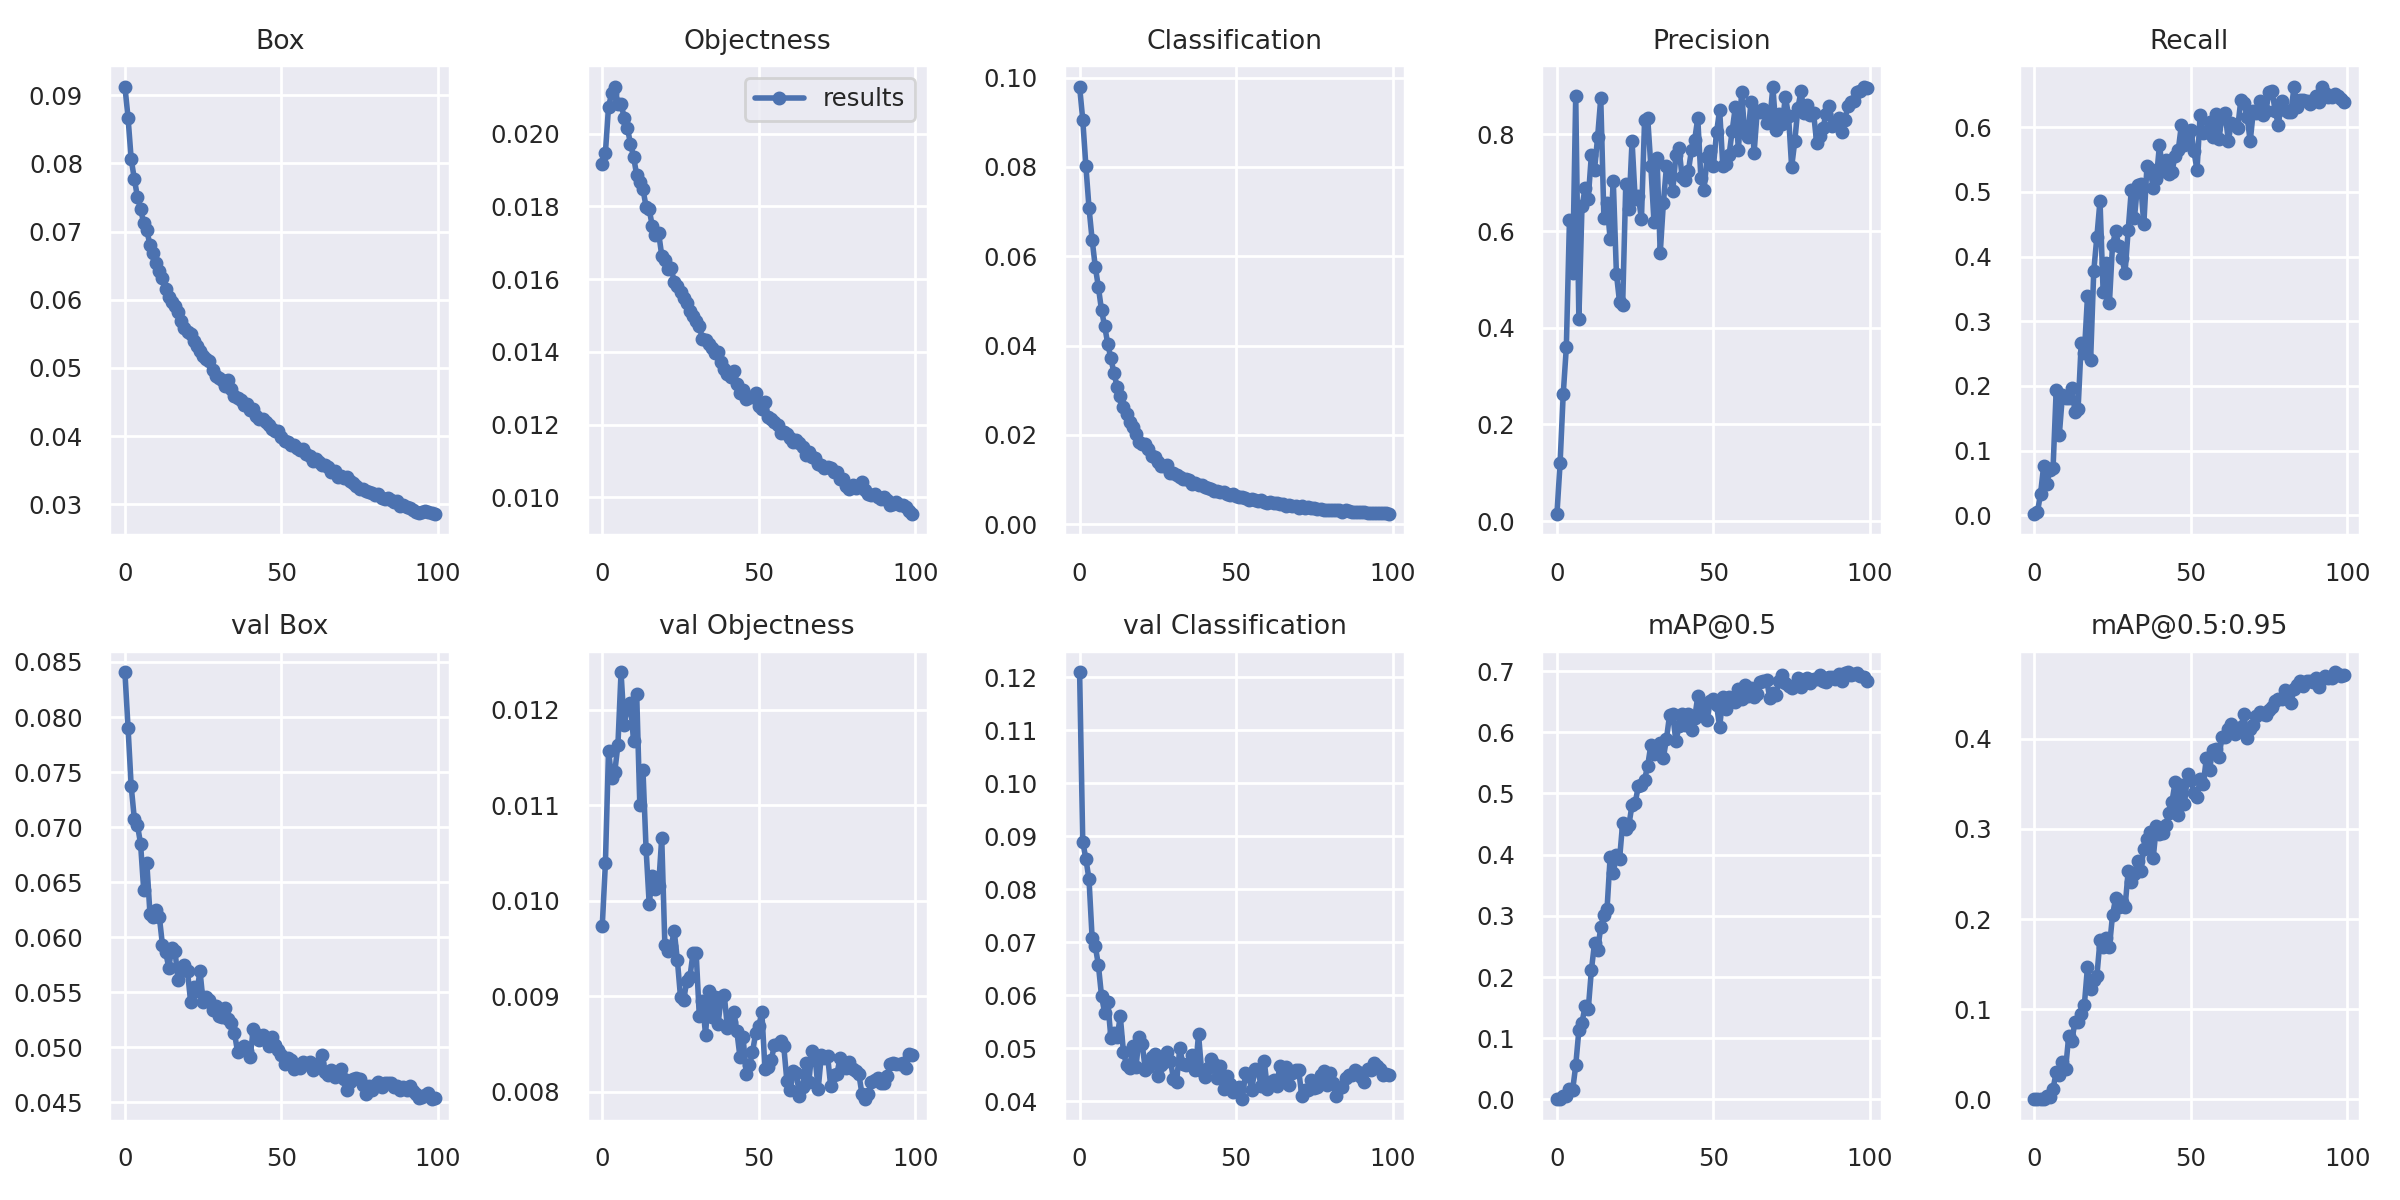
\includegraphics[width=0.9\linewidth]{Experiments/MoCA/results.png}\\
    \caption{Results on the MoCA Dataset}
    \label{fig8}
\end{figure}

\begin{figure}[ht]
\centering
\begin{subfigure}{0.7\linewidth}
    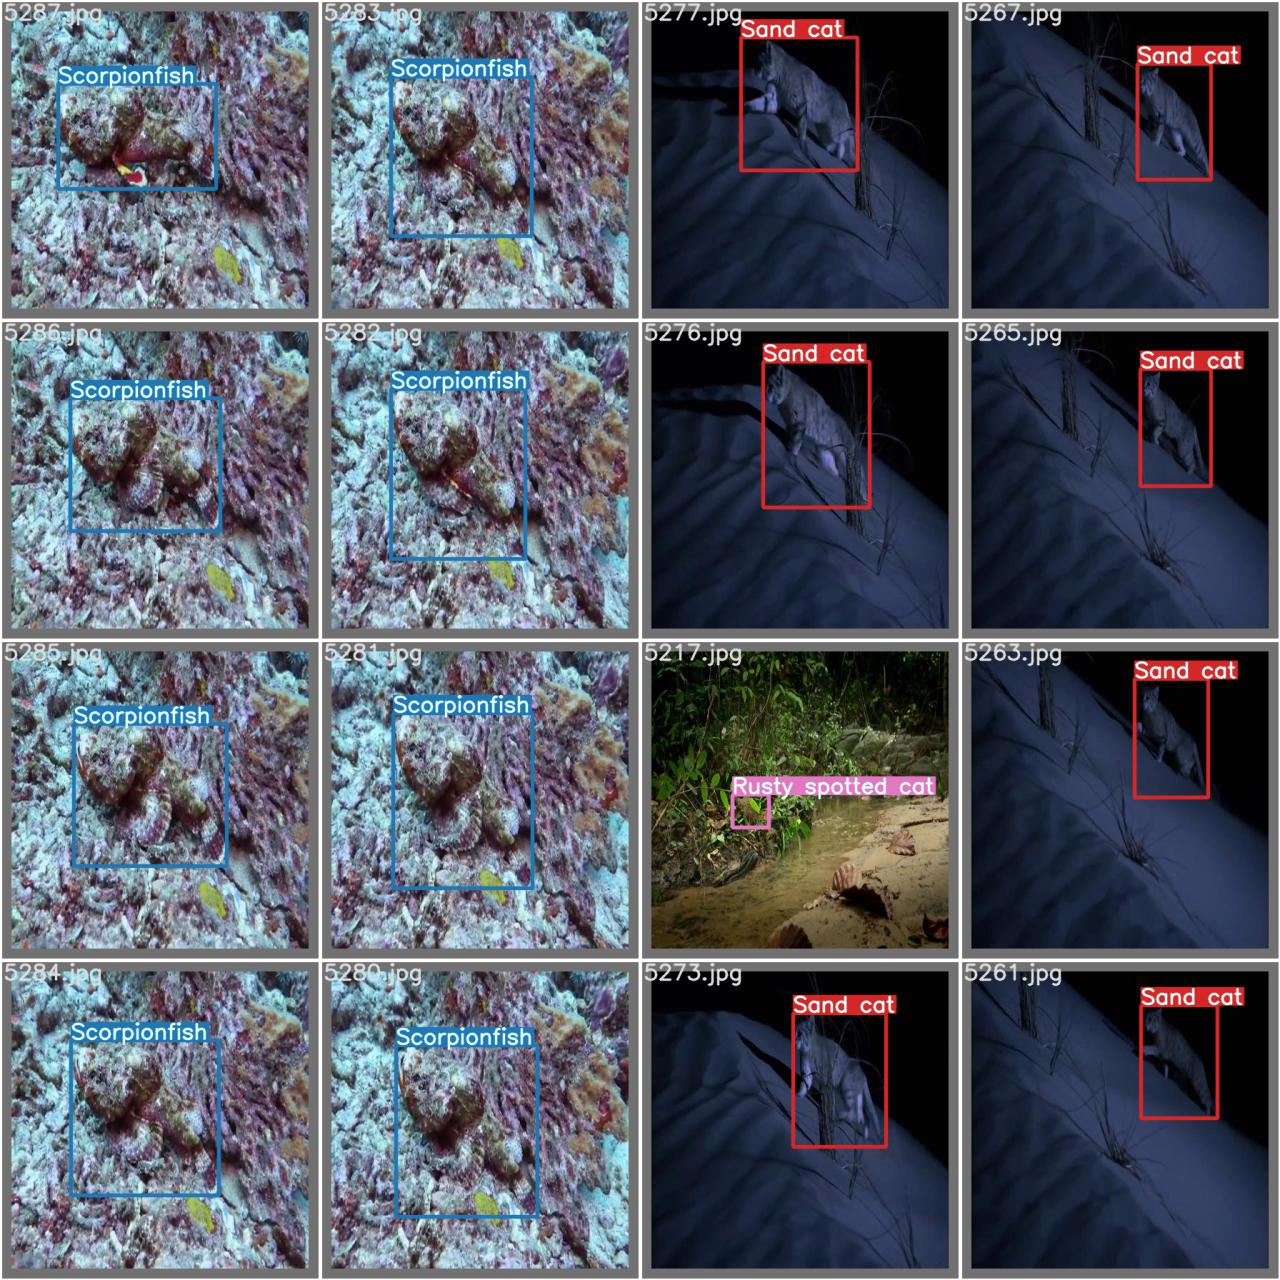
\includegraphics[width=1\textwidth]{Experiments/MoCA/test_batch1_labels.jpg}
    \caption{Test Batch Labels}
    \label{fig:moca_label}
\end{subfigure}
\hfill
\begin{subfigure}{0.7\linewidth}
    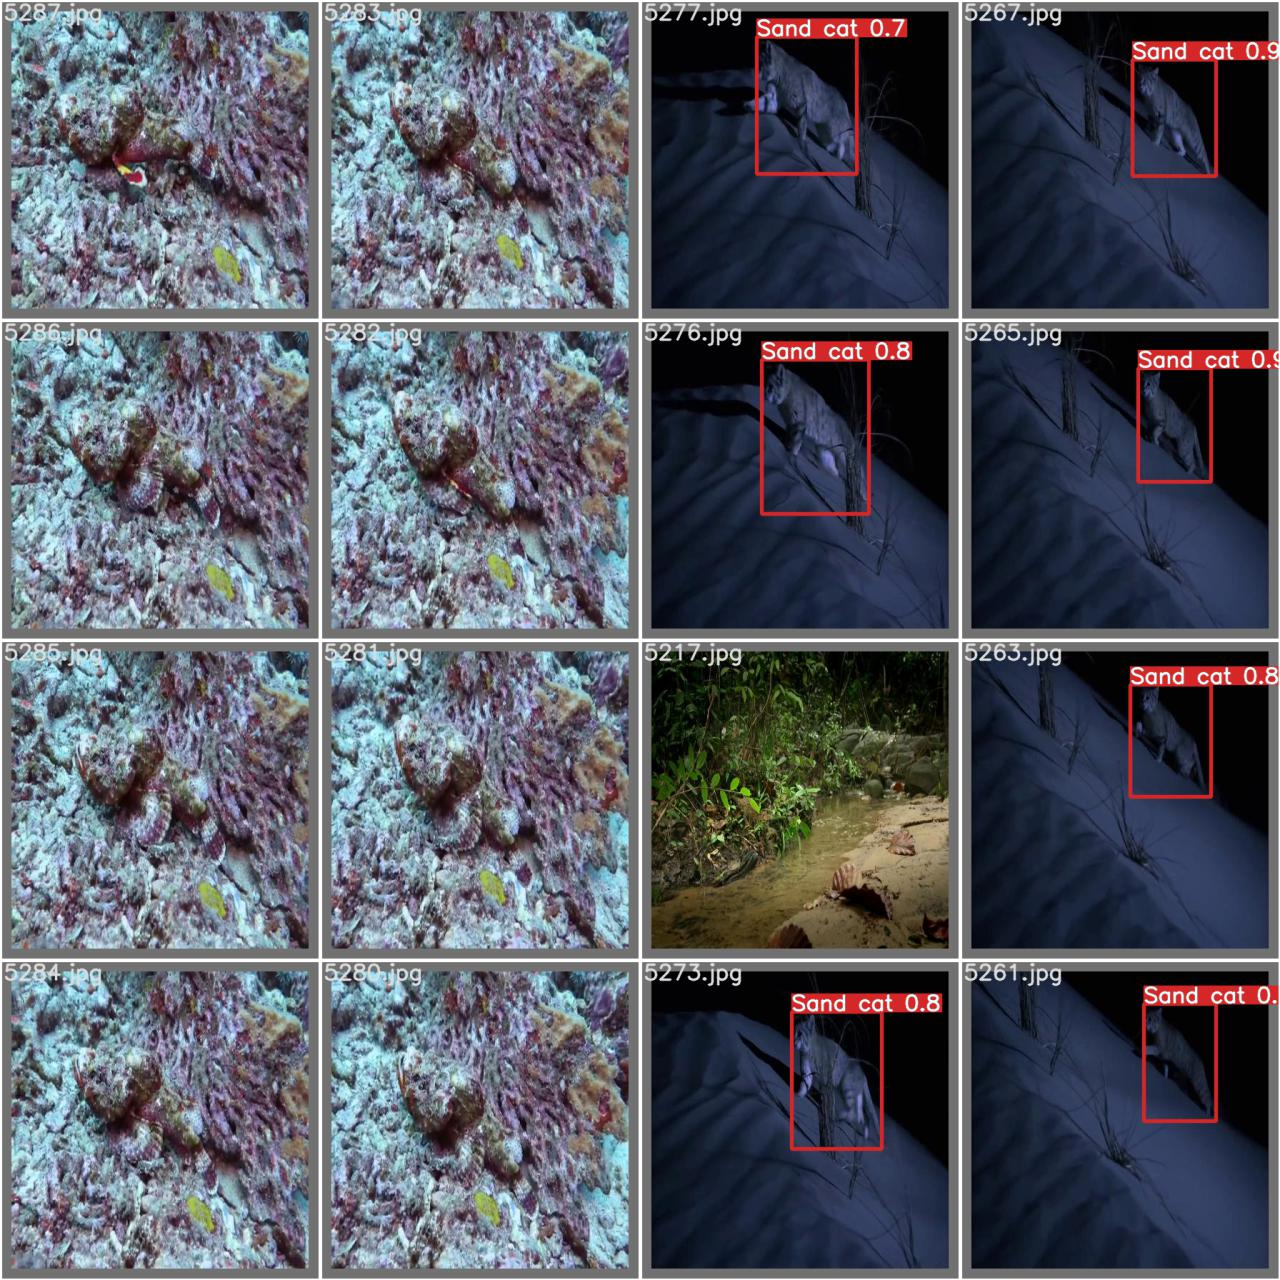
\includegraphics[width=1\textwidth]{Experiments/MoCA/test_batch1_pred.jpg}
    \caption{Test Batch Predictions}
    \label{fig:moca_pred}
\end{subfigure}
\caption{The actual labels \& the predicted labels on a test batch of the MoCA dataset by the YOLOv5s model}
\label{fig:moca}
\end{figure}
We can see that overall training is fast in this dataset and that our model learns bounding boxes of the camouflaged objects reasonably well in both training and test data. This could be due to temporal relationship between frames. The model also learns well whether an object exists within the frame or not (Objectness loss) and learns well to distinguish between classes (classification loss) extremely quickly. The mAP is also relatively high again owing to how similar the frames are. Although this may seem promising, a larger dataset would be needed to verify whether the model has `learned` or `memorized` the features. Figure \ref{fig:moca_pred} shows some of the predictions on the test set while Figure \ref{fig:moca_label} containing ground truths. 
% \newpage
\subsection{COD10K DATASET}
\begin{figure}[h]
    \centering
    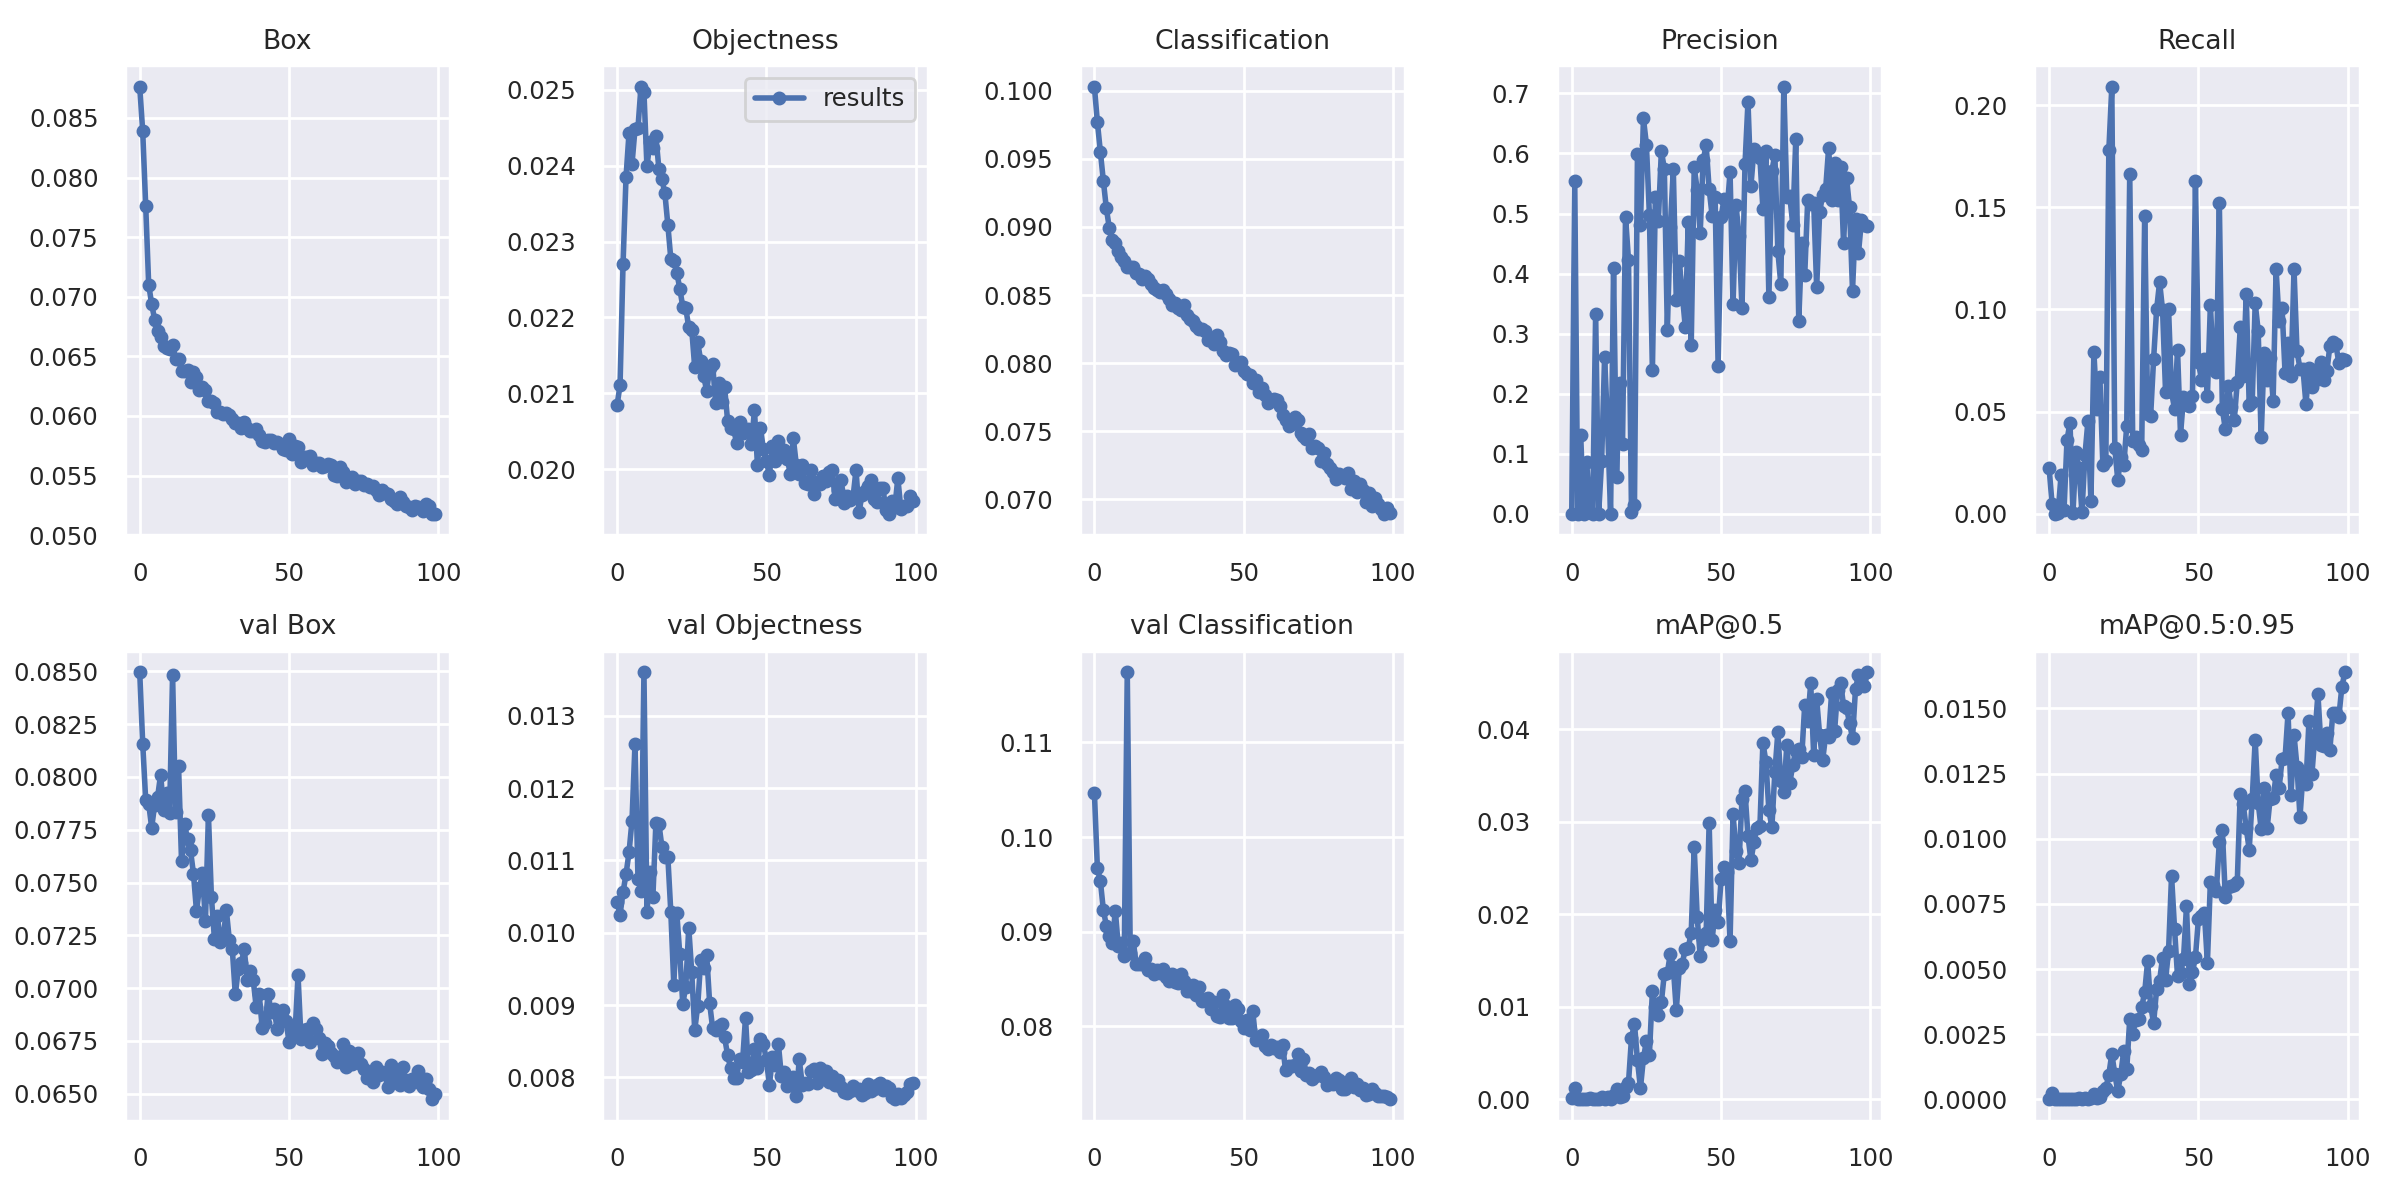
\includegraphics[width=0.9\linewidth]{Experiments/COD10K/results.png}\\
    \caption{Results on the COD10K Dataset}
    \label{fig10}
\end{figure}
The model trained on this dataset does regress it bounding boxes quickly and learns the classes of the objects as well however, it has failed to learn to detect the object within the images. This is the reason why the model although has a high precision has an extremely low recall leading to low mAP scores. This is possibly due to the similarities between the object that we want to detect and the environment. Figure \ref{fig:cod10k_pred} shows some of the results on the test set with Figure \ref{fig:cod10k_label} containing ground truths.
\begin{figure}[ht]
\centering
\begin{subfigure}{0.7\linewidth}
    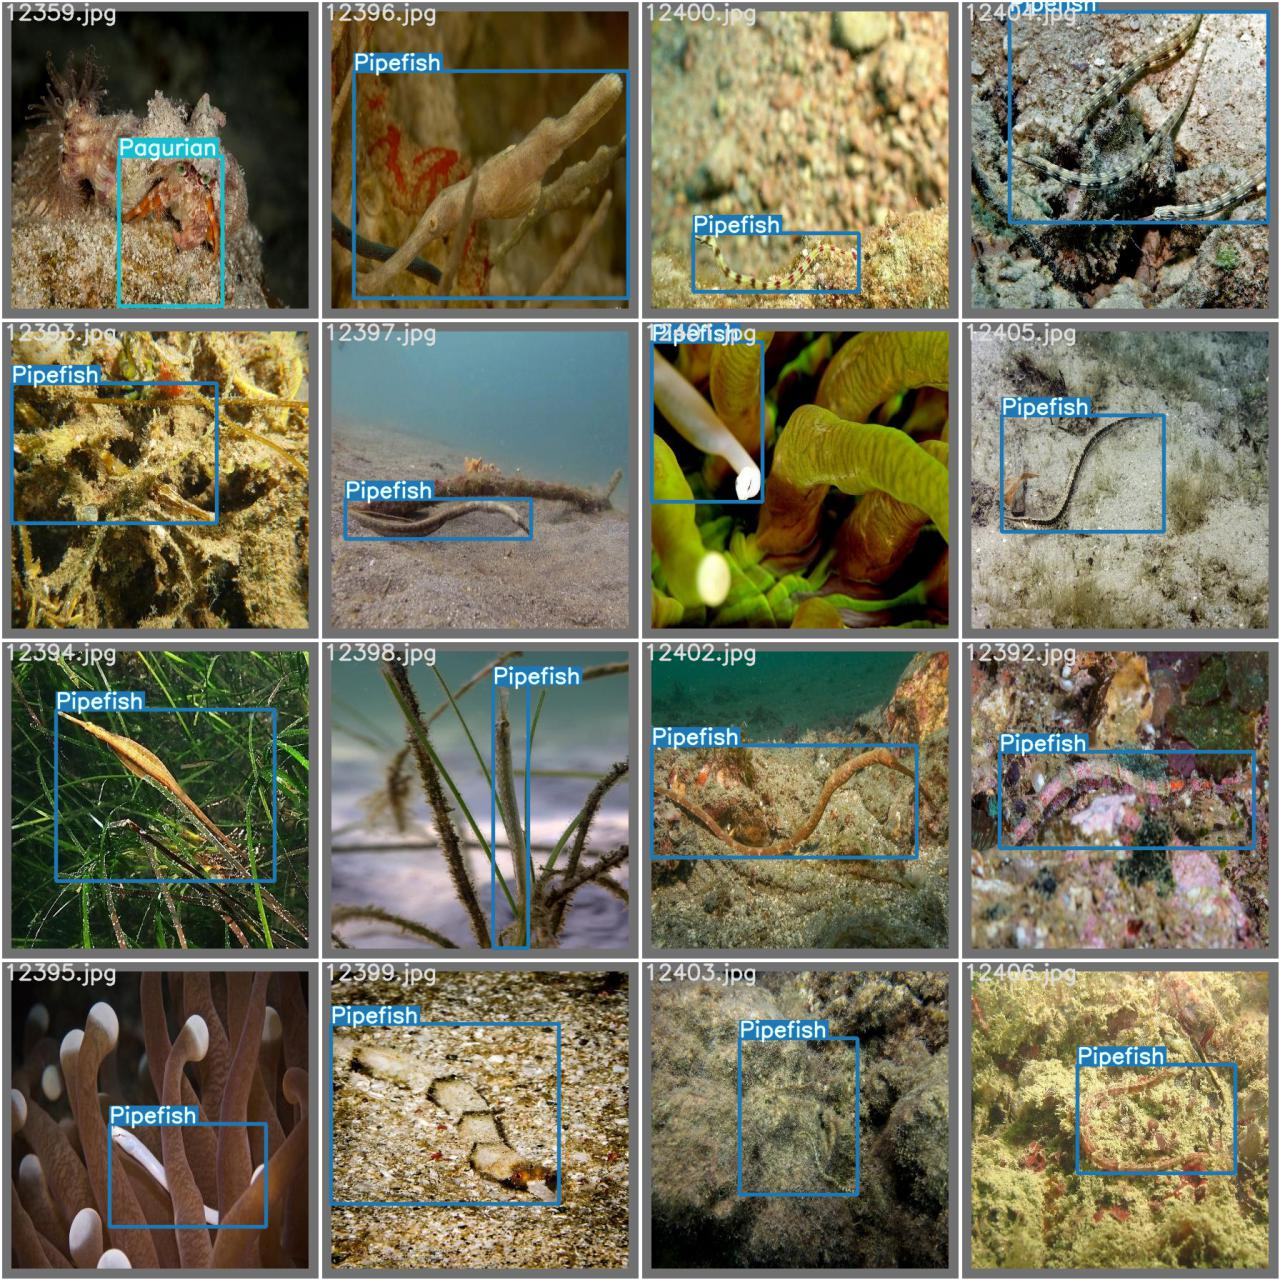
\includegraphics[width=1\textwidth]{Experiments/COD10K/test_batch2_labels.jpg}
    \caption{Test Batch Labels}
    \label{fig:cod10k_label}
\end{subfigure}
\hfill
\begin{subfigure}{0.7\linewidth}
    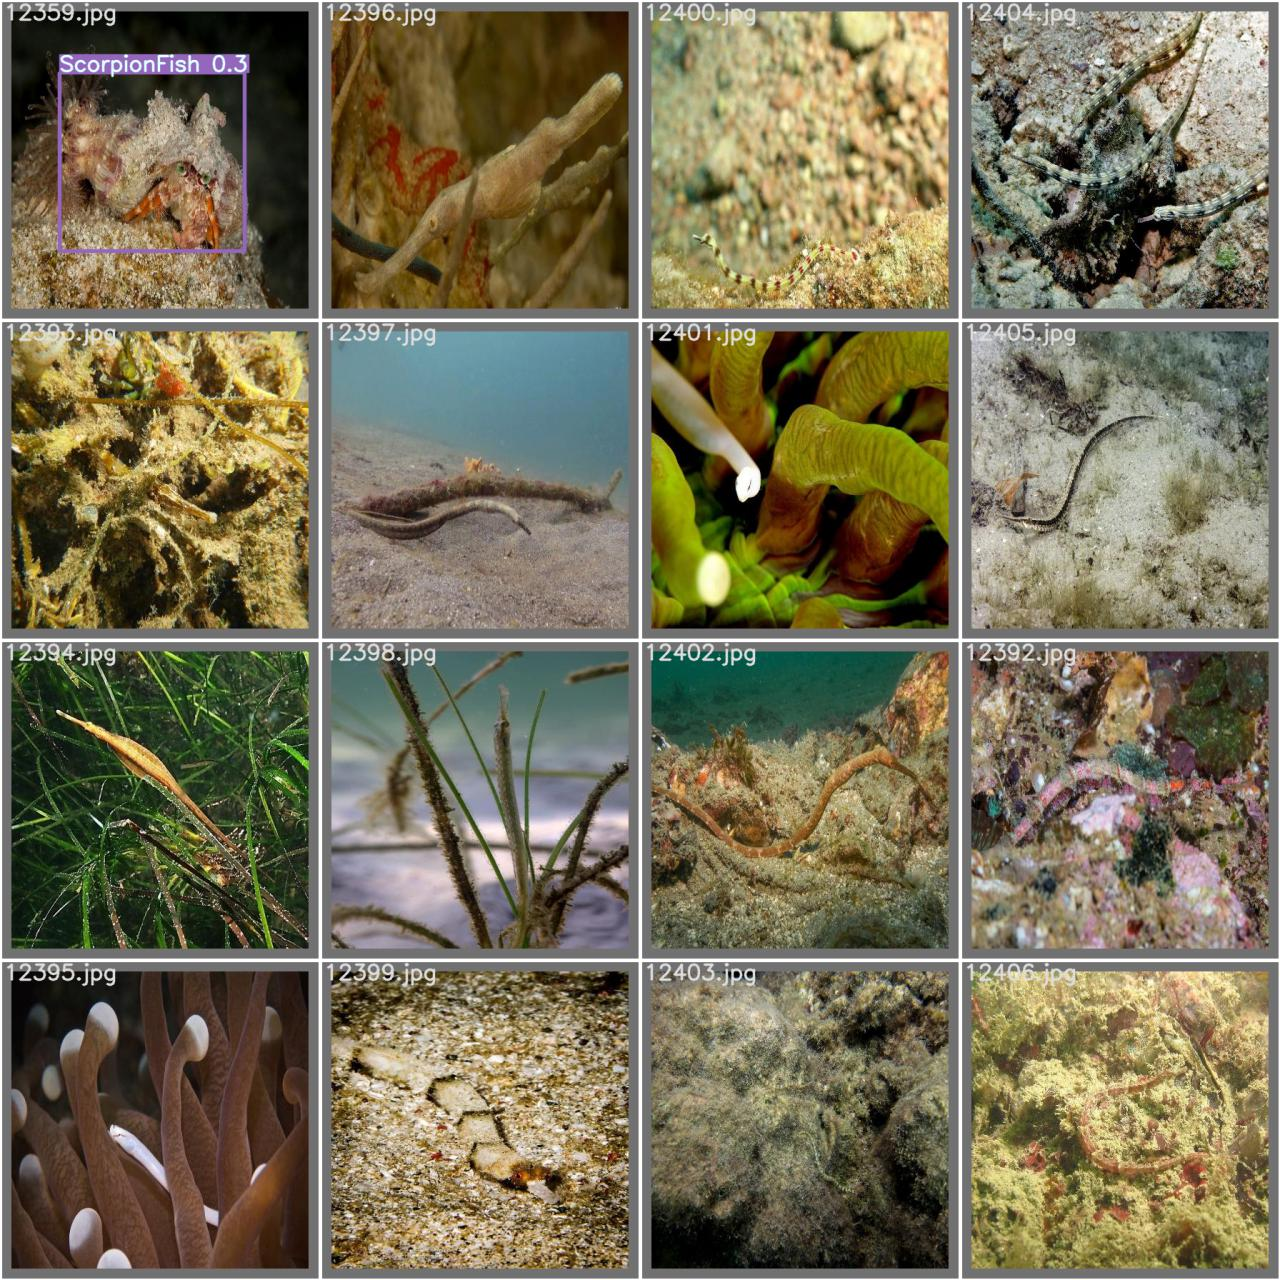
\includegraphics[width=1\textwidth]{Experiments/COD10K/test_batch2_pred.jpg}
    \caption{Test Batch Predictions}
    \label{fig:cod10k_pred}
\end{subfigure}
\caption{The actual labels \& the predicted labels on a test batch of the COD10K dataset by the YOLOv5s model}
\label{fig11}
\end{figure}
\newpage
\subsection{MERGED DATASET}
\begin{figure}[h]
    \centering
    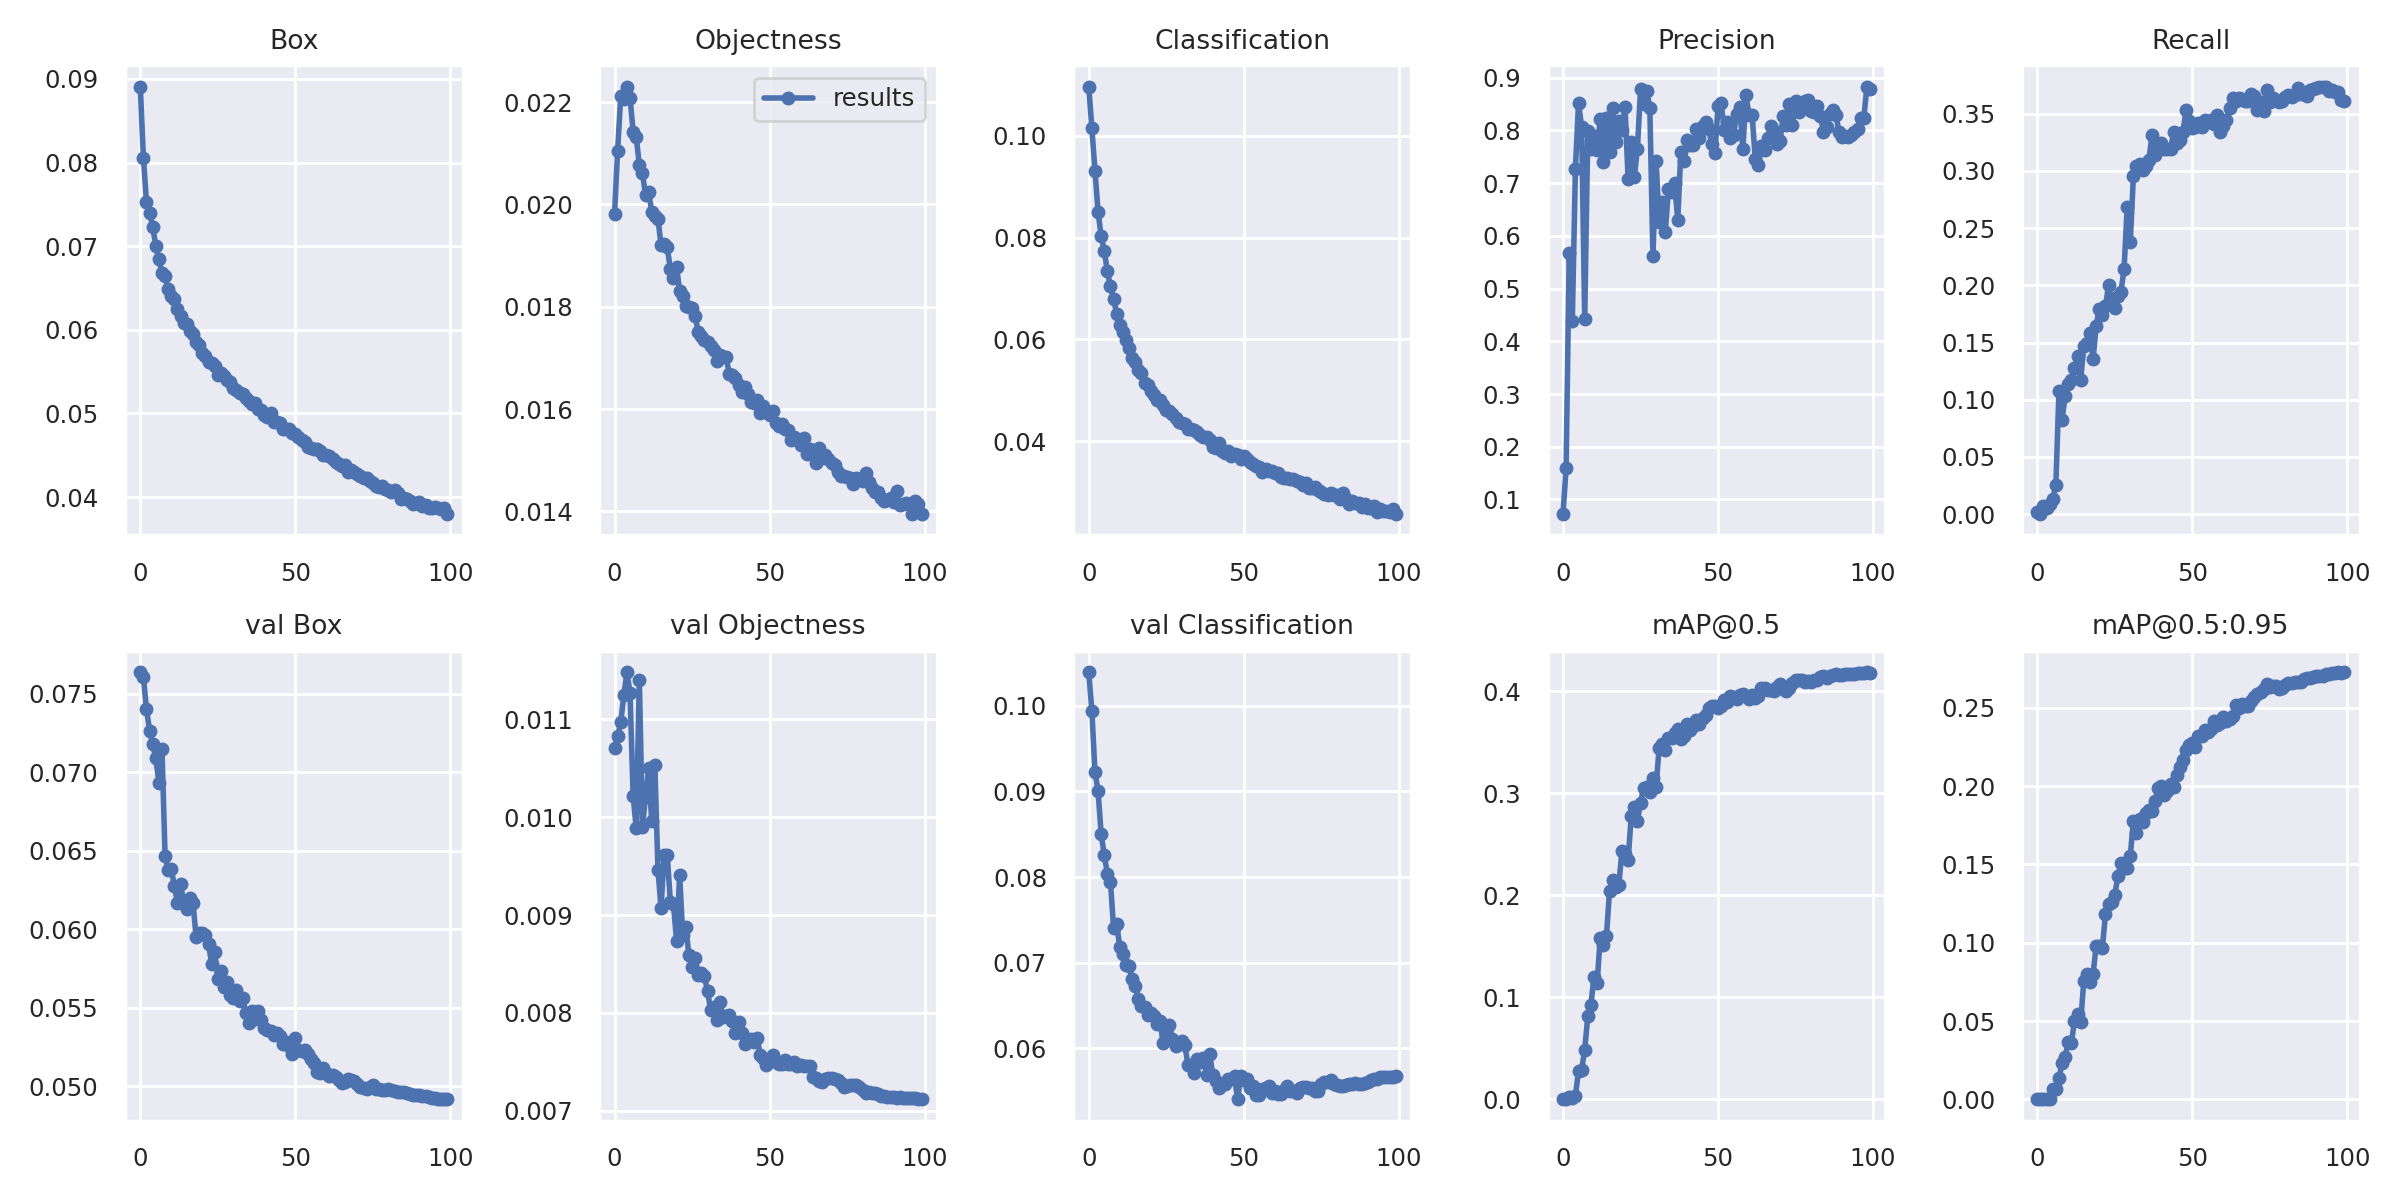
\includegraphics[width=0.9\linewidth]{Experiments/Merged/results.png}\\
    \caption{Results on the merged Dataset}
    \label{fig12}
\end{figure}
\begin{figure}[ht]
\centering
\begin{subfigure}{0.7\linewidth}
    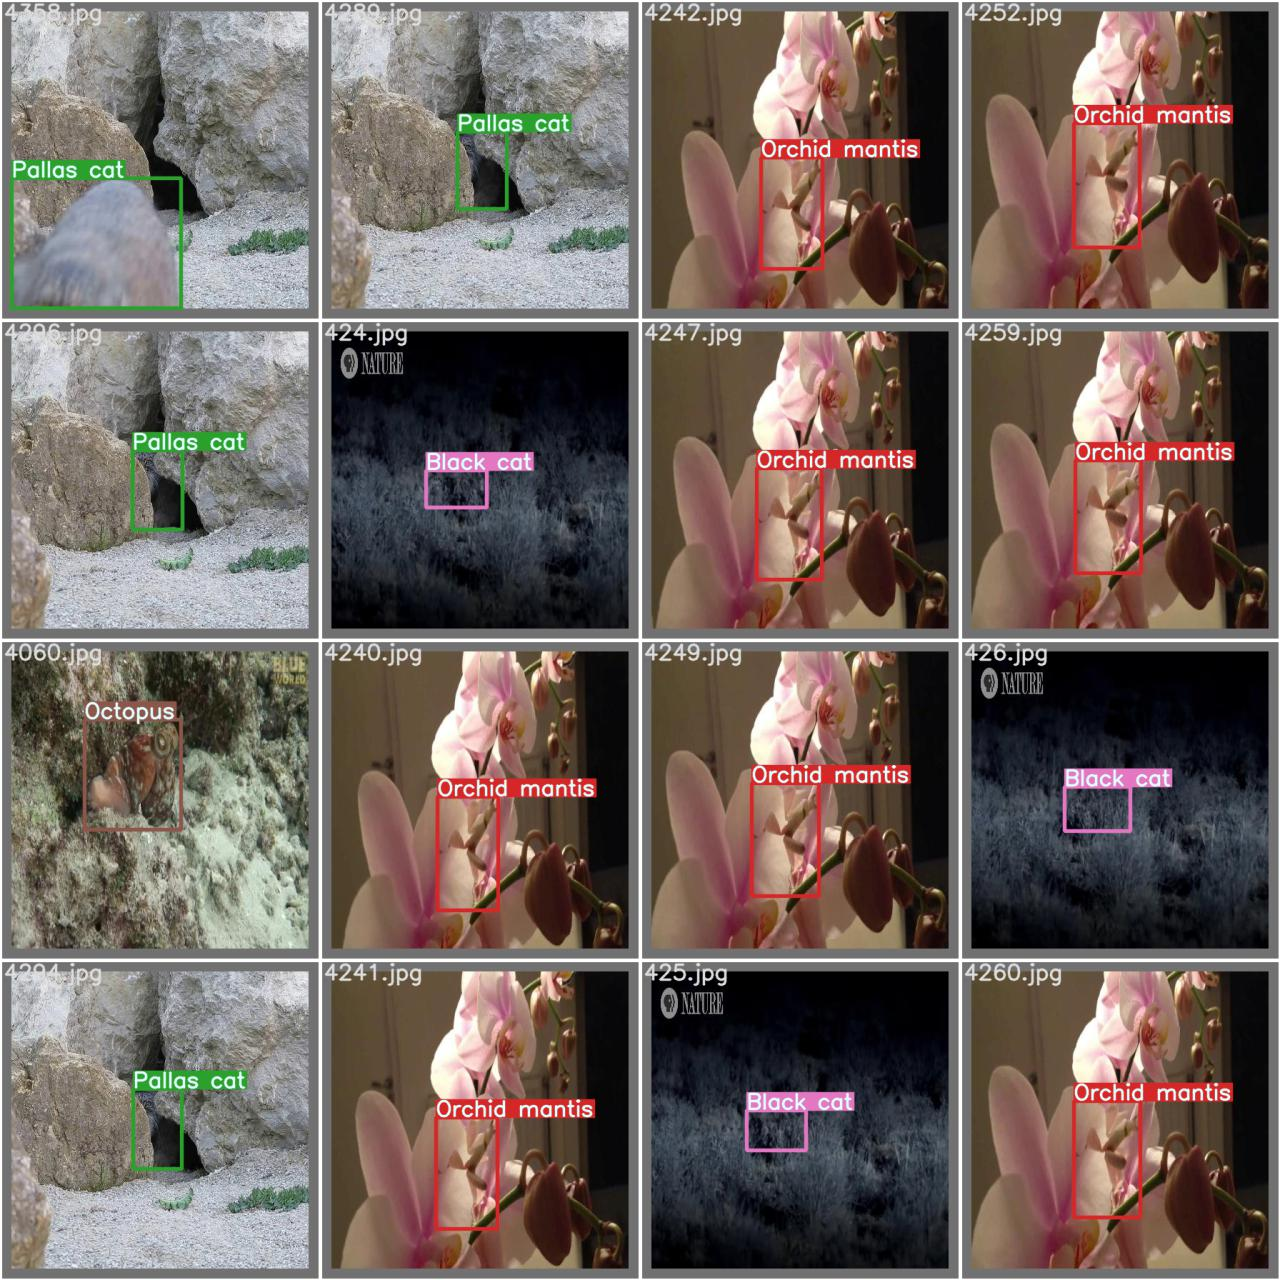
\includegraphics[width=1\textwidth]{Experiments/Merged/test_batch2_labels.jpg}
    \caption{Test Batch Labels}
    \label{fig:merged_label}
\end{subfigure}
\hfill
\begin{subfigure}{0.7\linewidth}
    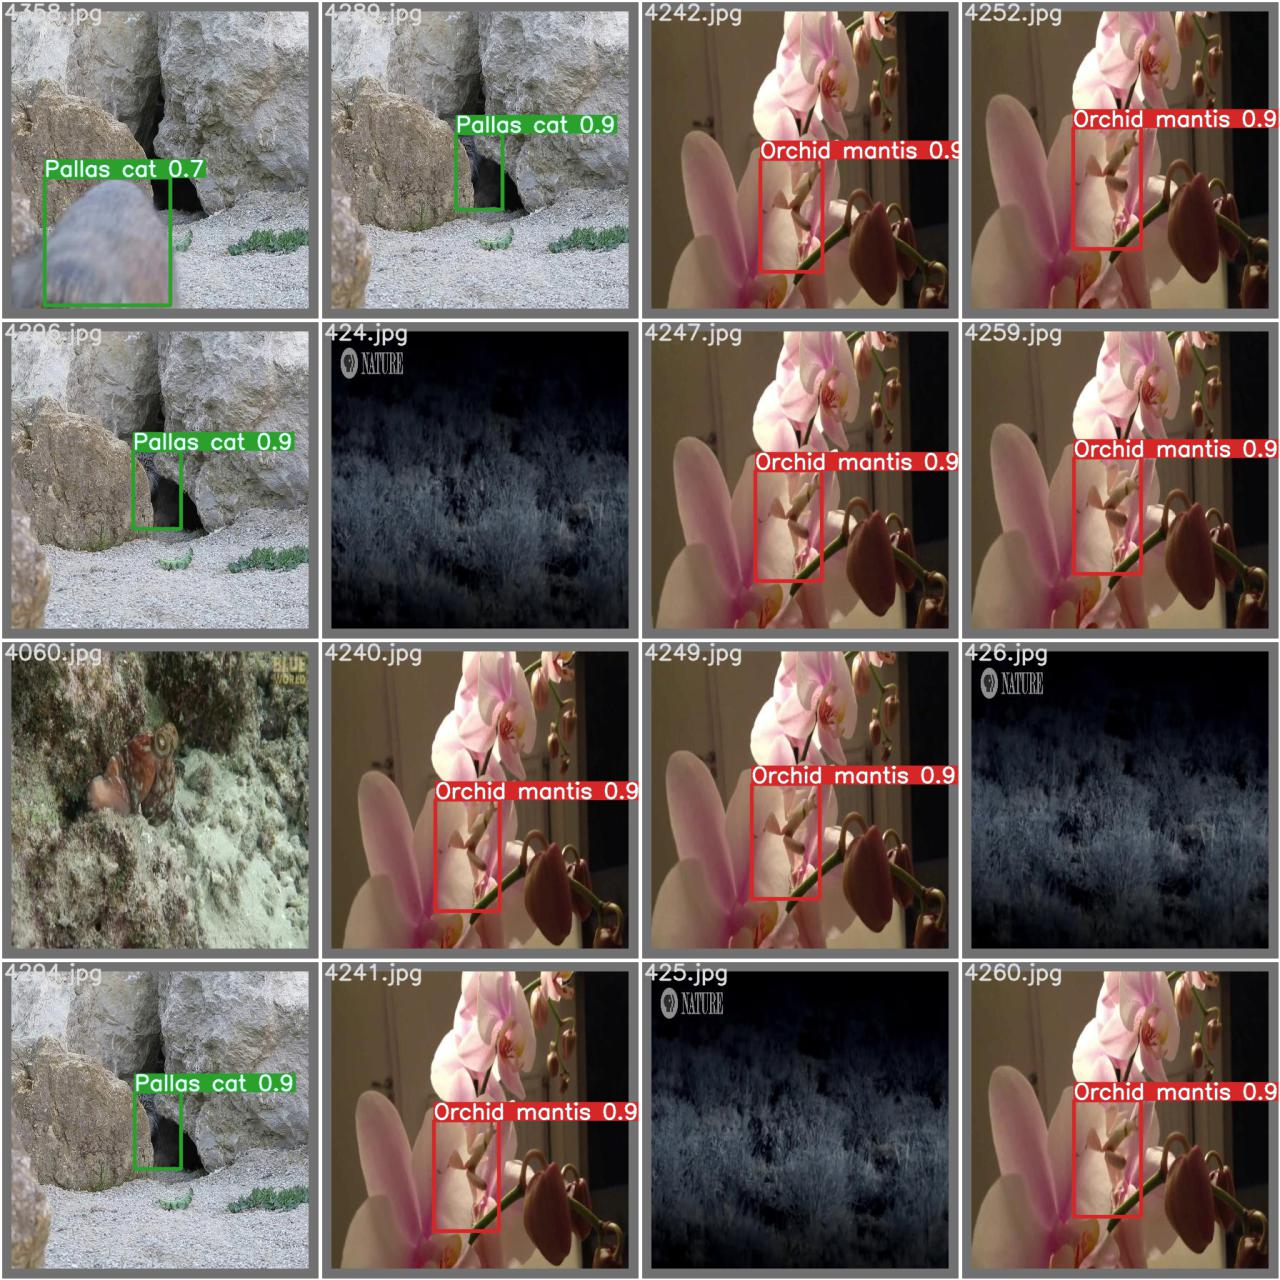
\includegraphics[width=1\textwidth]{Experiments/Merged/test_batch2_pred.jpg}
    \caption{Test Batch Predictions}
    \label{fig:merged_pred}
\end{subfigure}
\caption{The actual labels \& the predicted labels on a test batch of the Merged dataset by the YOLOv5s model}
\label{fig13}
\end{figure}
In this dataset, we can see overall a mixture of the results that we found in the two datasets separately. The mAP is higher than that of COD10K but lower than that of MoCA dataset. Merging the two datasets allowed the model to have more data for 10 classes, which could lead to better detections within those categories. Bounding box detection, seeing whether an object is within frame or not and classification loss and precision have similar trends as MoCA dataset. Recall is higher than on COD10K alone but lower than MoCA suggesting that we need more data for classes on objects just in COD10K. Figure \ref{fig:merged_pred} shows some of the predictions on the test set while Figure \ref{fig:merged_label} containing ground truths. 
\newpage
\subsection{DISCUSSION}

% Please add the following required packages to your document preamble:
% \usepackage{graphicx}
\begin{table}[ht]
\centering
\resizebox{\linewidth}{!}  & 47.36\%     \\ \hline
\multicolumn{1}{|l|}{COD10K \ref{fig10}}      & \multicolumn{1}{l|}{4.615\%} & 1.638\%    \\ \hline
\multicolumn{1}{|l|}{MoCA+COD10K \ref{fig12}} & \multicolumn{1}{l|}{41.86\%}  & 27.25\%     \\ \hline
\end{tabular}%
}
\caption{Summary of the Performance of the YOLOv5s Model}
\label{tab:my-table3}
\end{table}

Based on the Table \ref{tab:my-table3}, and Figures \ref{fig8},\ref{fig10},\ref{fig12} we can conclude that the YOLOv5s model had the best performance in terms of mAP both @.5 and @.5:.95 as well as recall,  on the MoCA Dataset, followed by the Merged Dataset and then COD10K Dataset. The reason for this is that the MoCA Dataset is a dataset formed from video frames and video data has a temporal relationship as well a lot of redundancy. Furthermore, from figures \ref{fig:moca_label},\ref{fig:cod10k_label}, and \ref{fig:merged_label}, we can see that the MoCA dataset has the most similar images whereas the COD10K has the least similar images. Consequently, if the model is able to detect the one instance of an object, it should be able to detect other instances of that same object. In Figure \ref{fig:moca_pred}, we can see that the model was able to detect all instances of the Sand Cat but no instance of the Scorpion. We can see a similar trend in \ref{fig:merged_pred} as well. However, in case of \ref{fig:cod10k_pred}, we can see that the model is only able to predict one bounding box out of the 16 images and that too with the incorrect label despite of the fact that 15 out of the 16 images had the same label, Pipefish. 

\section{CHALLENGES}
The biggest challenge faced by Camouflaged Object Detection is the lack of annotated data. Currently, either the bounding box information is missing such as in the MoCA or we have the bounding box information but the labels are missing such as CHAMELEON or both in the case of COD10K. Therefore, we were only to able to use 20\% of the MoCA Dataset and 50\% of the COD10K Dataset. Another challenge that we face in COD is the conversion of segmentation to bounding boxes. The thing that makes this conversion challenging is occlusion. This is because we may find multiple bounding boxes in one image even though they correspond to one partially object. We chose to resolve this by finding the minimum enclosure box for all the bounding boxes but this approach is appropriate only work if there is only one object in the image.

\section{CONCLUSION AND FUTURE WORK}
Currently, we only used the YOL0v5s model but we would like to extend this work by also using different YOLOv5 models such as the Y0LOv5 medium (YOLOv5m) and Y0LOv5 large (YOLOv5l) in order to understand how different YOLOv5 models compare. In addition, we would to like use different models from the YOLO series such as the YOL0X and YOLOF to have more baseline results to compare with then the same models are tested on synthetic data. The YOLOv5s model performed reasonably well on the MoCA Dataset because of the temporal relationship between video frames and as well redundancy and fairly well on the merged dataset for the same reason and due to more data for 10 classes. In the future, we would like to test how this hold hypothesis holds for classes with limited data by generating more samples of the same class by data augmentation. Furthermore, if we want the data centric approach to achieve better results, more real and similar data needs to be collected so that our model can learn better and more general representation of each classes. The currently available data also needs to be annotated with proper labels so that it can be used in object detectors.





% \section{MODEL \& EXPERIMENTS}

% Please add the following required packages to your document preamble:
% \usepackage{graphicx}

 




% Please add the following required packages to your document preamble:
% \usepackage{graphicx}



% \section{Results \& Discussion}
% \section{Future Work}



\bibliography{references}
\bibliographystyle{plain}

\end{document}


